\section{Model Based Approach}
\label{sec:modelbased}
We now propose a model for SQL-on-Hadoop engines that builds on the insights described in the previous section. We will describe the model for Apache Hive on Hadoop2 MR and Apache Spark. We will show that even though the model is simple, it is a sufficient approximation to generate good recommendations. 

\subsection{Algorithm}
To model the behavior of a query, we need to know the characteristics of the data processed by the query. This includes the input data size and the output data size for each MR stage of the query processing pipeline. One way to estimate this is to use statistics such as sizes of the tables, number of distinct values for each attribute and histograms that will enable us to estimate selectivities of various operators in the query. However, getting accurate data statistics in a big data environments is very often a challenge. Since we are mainly concerned with ETL queries, we can exploit the fact that these queries are run periodically. SQL-on-Hadoop engines collect a lot of metric and configuration information from the jobs that are executed in the system. The overall approach is thus to use the data collected during a run of the query as inputs to our algorithm to recommend good configuration parameters for future runs of the query. The job metrics and parameters used by the algorithm are listed in Table~\ref{table:job_metrics}. The algorithm also takes as input information about the machine instance type and configuration, as listed in Table~\ref{table:inst_conf}. Besides these, there are some global parameters that can be used to tune the algorithm, as listed in Table \ref{table:global_params}.

\eat{
The inputs to the algorithms are:
\begin{enumerate}
    \item[$\bullet$] Job Parameters: These are the key input parameters of the job that effect performance and cost. Table \ref{table:job_params} defines these job parameters.
    \item[$\bullet$] Instance configuration: Table \ref{table:inst_conf} defines the machine configuration.
    \item[$\bullet$] Global Parameters: These are some of the global parameters that can be used to tune the algorithm. These are defined in Table \ref{table:global_params}.
\end{enumerate}
}

\begin{table}
\begin{tabular}{ |l|p {4.5 cm}| } 
 \hline
 Parameters & Description \\ 
 \hline
 mapperTime  & Total mapper time in seconds   \\ 
 numOfMapper & Number of map tasks \\ 
 mapperMemory & Container memory for map tasks  \\ 
 splitSize & Input Split Size \\
 mapperInputBytes & Map input in bytes \\
 mapperOutputBytes & Map output in bytes \\
 mapperOutputRecords & Number of Map output records \\
 reducerTime & Total reducer time in seconds \\
 numOfReducer & Number of reduce tasks \\
 bytesPerReducer & Corresponds to Hive parameter \textit{hive.exec.reducers.bytes.per.reducer} \\
 reducerMemory & Container memory for reduce tasks \\
 ioSort & Total amount of buffer memory in mega bytes to be used for sorting. Corresponds to Hadoop parameter \textit{mapreduce.task.io.sort.mb} \\
% spilledMapRecords & Number of records spilled in Map tasks  \\
 spilledMapBytes & Bytes spilled in Map tasks  \\
 spilledRedBytes & Bytes spilled in Reduce tasks  \\
 \hline
\end{tabular}
\caption{Job metrics and parameters}
\label{table:job_metrics}
\end{table}

\begin{table}[h]
\begin{tabular}{ |l|p {4.5 cm}| }
 \hline
 Parameters & Description \\ 
 \hline
 nodeMemory  & Total available memory per node for MR job   \\ 
 cpuPerNode & Number of CPUs per node \\ 
 vCpuPerNode & Number of vCPUs per node  \\
 eCPU & computing units per node similar to Amazon ECU \\
 \hline
\end{tabular}
\caption{Instance configuration}
\label{table:inst_conf}
\end{table}

\begin{table}[h]
\begin{tabular}{ |p {1.8 cm}|p {3.5 cm}|p {1 cm} | } 
 \hline
 Parameters & Description & Default\\ 
 \hline
 ioSortFrac & Size of ioSort buffer specified as fraction of mapper memory & 0.4 \\
 maxIOSort & Maximum value for \textit{mapreduce.task.io.sort.mb} & 2047 \\
 reducerFrac & Fraction of Reducer memory to be used as buffer & 0.4 \\ 
 minMapTime & Minimum time that a mapper should take & 60s \\
 minRedTime & Minimum time that a reducer should take & 60s \\ 
 \hline
\end{tabular}
\caption{Global Parameters}
\label{table:global_params}
\end{table}


Algorithm \ref{alg:optres} optimizes cumulative resource utilization of a SQL query. It can be seen from Equation~\ref{eqn:totalresource} that resource utilization can be reduced by decreasing either the memory usage or time taken for processing. The algorithm thus aims to reduce the memory usage without increasing the time. Insight~\ref{insight:mem} indicates that memory usage can reduced without adverse effect by increasing parallelism if necessary. Insight~\ref{insight:parallelism} further says that parallelism should not be increased indiscriminately. Thus the algorithm maintains a lower bound on the mapper and reducer time ($minMapTime$ and $minRedTime$). It first computes the rate of processing of the mappers (line 1), based on the time metric of the previous run and uses it to compute the splitSize, such that each mapper takes at least $minMapTime$ (line 2). It then computes the $ioSort$, such that the output of each mapper fits in that buffer to avoid spills as per Insight~\ref{insight:spill} (line 3--4). The output size of a mapper is estimated using metrics from the previous run (line 3). The mapper memory is computed from the $ioSort$, using the global parameter $ioSortFrac$ (line 5). Similar computations are done to determine the reducer parallelism ($bytesPerReducer$) and $reducerMemory$ (lines 6--9). Finally, the expected resource usage based on the new parameters is computed (line 10--12).

\renewcommand{\algorithmicrequire}{\textbf{Input:}}
\renewcommand{\algorithmicensure}{\textbf{Output:}}
\renewcommand{\algorithmiccomment}[1]{// #1}
\begin{algorithm}
	\caption{OptResource}\label{alg:optres}
	\begin{algorithmic}[1]
		\footnotesize
		\REQUIRE  $\mathcal{P}$ is the job metrics and parameters (defined in table \ref{table:job_params}) from one run, $I$  is instance configuration (defined in Table \ref{table:inst_conf}) on which $\mathcal{P}$ is collected, $\mathcal{G}$ is the global parameters defined in Table \ref{table:global_params}
		\ENSURE New job parameters $\mathcal{P}_{new}$ and the expected cumulative resource usage $expectedResUsage$ after optimization.
		\STATE $mapTimePerByte \gets mapperTime/(mapperInputBytes + spilledMapBytes)$
		\STATE $\mathcal{P}_{new}.splitsize \gets minMapTime/mapTimePerByte$
		\STATE $mapOutPerSplit \gets \mathcal{P}_{new}.splitsize \times (mapperOutputBytes/mapperInputBytes)$
		\STATE $\mathcal{P}_{new}.ioSort \gets mapOutPerSplit$
		\STATE $\mathcal{P}_{new}.mapperMemory \gets \mathcal{P}_{new}.ioSort / ioSortFrac$
		\STATE $redTimePerByte \gets reducerTime/(mapperOutputBytes + spilledRedBytes)$
		\STATE $dataPerRed \gets minRedTime/redTimePerByte$
		\STATE $\mathcal{P}_{new}.bytesPerReducer \gets dataPerRed \times (mapperInputBytes/mapperOutputBytes)$
		\STATE $\mathcal{P}_{new}.reducerMemory \gets dataPerRed / reducerFrac$
		\STATE $numMappers \gets mapperInputBytes/\mathcal{P}_{new}.splitsize$
		\STATE $numReducers \gets mapperInputBytes/\mathcal{P}_{new}.bytesPerReducer$
		\STATE $expectedResUsage \gets numMappers \times minMapTime \times \mathcal{P}_{new}.mapperMemory  + numReducers \times minRedTime \times \mathcal{P}_{new}.reducerMemory$
		\STATE \RETURN $\mathcal{P}_{new}, expectedResUsage$
	\end{algorithmic}
\end{algorithm}



%\begin{algorithm}
%\caption{checkFit} \label{checkfit}
%\begin{algorithmic}[1]
%\footnotesize
%\REQUIRE $\mathcal{P}$ is the job parameters (defined in \ref{table:job_params} ), $\mathcal{I}$  is instance configuration (defined in \ref{table:inst_conf})
%\ENSURE Returns \textit{true} if $\mathcal{P}$ can fit into $\mathcal{I}$, otherwise \textit{false}.
%
%\STATE newMemPerCore $\gets \mathcal{I}.nodeMemory / \mathcal{I}.vCpuPerNode$
%\IF {newMemPerCore $> \mathcal{P}.mapperMemory$ and newMemPerCore $> \mathcal{P}.reducerMemory$}
%\RETURN \textit{true}
%\ELSE
%\RETURN \textit{false}
%\ENDIF
%\end{algorithmic}
%\end{algorithm}

\subsection{Results}
We evaluated the effectiveness of $OptResource$ method by running experiments on real workloads. The experiments were carried out for a HIVE on MR engine for a workload consisting of 4 real customer queries. 
Figure \ref{fig:modelbasedresult} shows the benefit predicted by our model and the actual observed benefit for these queries. The results show that the algorithm leads to significant savings in the cumulative resource usage cost, ranging from 70\% for $q3$ to 90\% for $q2$. Further, the actual savings closely match the predicted savings indicating that the model is reasonably accurate.

\begin{figure}[h]
	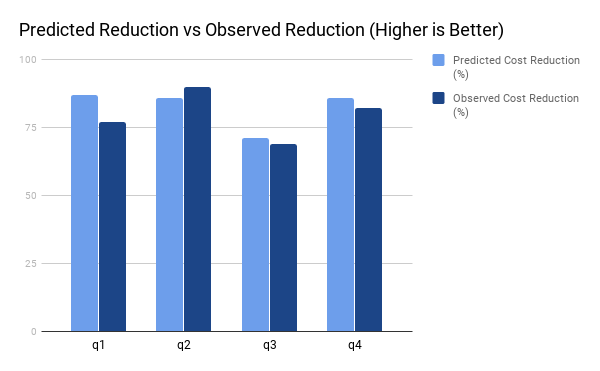
\includegraphics[width=\linewidth]{chart.png}
	%\vspace*{-15pt}
	\caption{Model Based Result: Predicted reduction in cost versus Actual reduction in cost for HIVE on MR queries}
	\label{fig:modelbasedresult}
\end{figure}

We also evaluated effectiveness of the same technique on SparkSQL. Algorithm for it is very similar to $OptResource$ and we are skipping it for brevity. We ran it on 3 real world SparkSQL customer queries. Figure \ref{fig:modelbasedresultspark} shows that the predicted percent reduction in cost matches that of actual reduction is cost observed with very high accuracy.

\begin{figure}[h]
	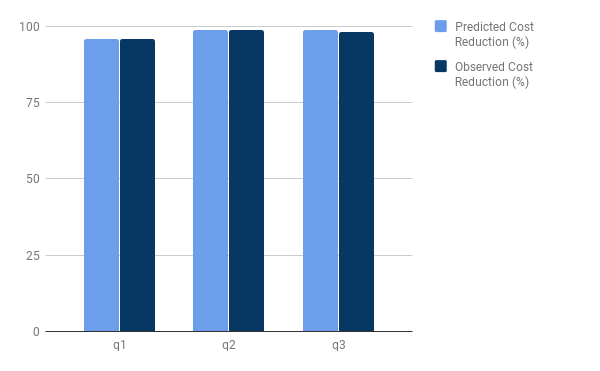
\includegraphics[width=\linewidth]{chart_spark.png}
	%\vspace*{-15pt}
	\caption{Model Based Result: Predicted reduction in cost versus Actual reduction in cost for SparkSQL queries}
	\label{fig:modelbasedresultspark}
\end{figure}